\emph{Aclaraciones:}
\begin{itemize}
 \item En los gráficos, el eje X representa el número de segmento
 \item En algunos gráficos, la cantidad de segmentos es variable. Creemos que esto sucede, ya que el número de re-transmisiones varía en cada corrida. La re-transmisión puede ocurrir por \emph{drop} o por \emph{timeout}.
\end{itemize}


\subsection{Sin pérdida de paquetes ($p$ = 0)}

\subsubsection{Varianza baja, delay bajo}

\begin{figure}[H]
\begin{minipage}{0.5\linewidth}
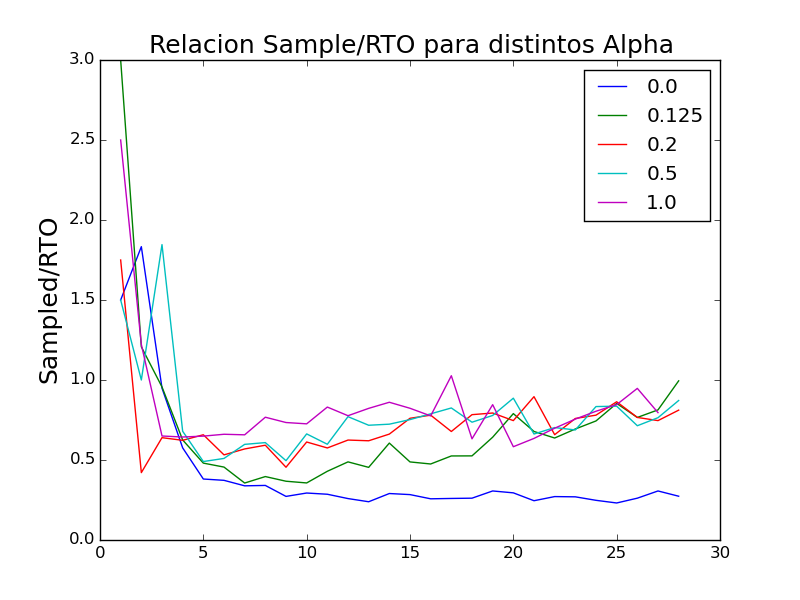
\includegraphics[width=\linewidth]{../graficos/alphad01var2drop0.png}
\caption{Relación Sample/RTO, $\beta$ = 0.25}\label{fig:alpha-var2-drop0}
\end{minipage}
\hfill
\begin{minipage}{0.5\linewidth}
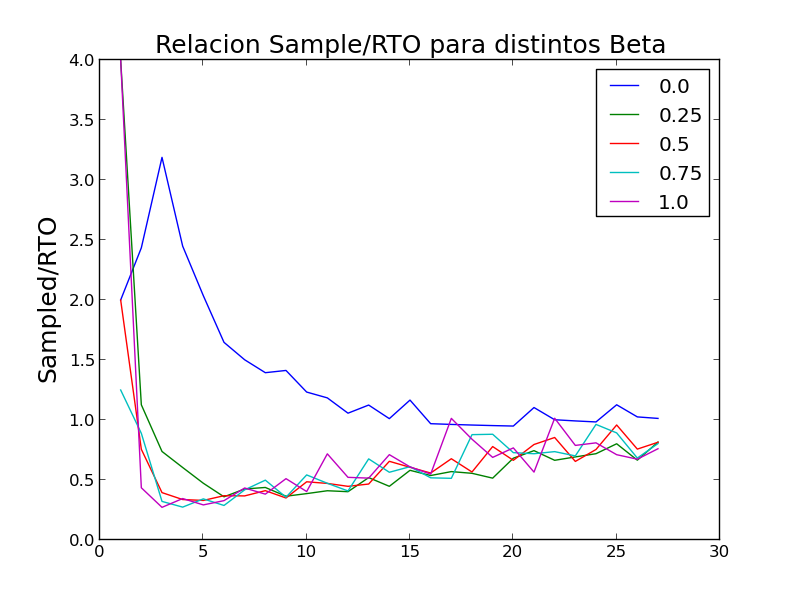
\includegraphics[width=\linewidth]{../graficos/betad01var2drop0.png}
\caption{Relación Sample/RTO, $\alpha$ = 0.125}\label{fig:beta-var2-drop0}
\end{minipage}
\end{figure}

\subsubsection{Varianza alta, delay bajo}

\begin{figure}[H]
\begin{minipage}{0.5\linewidth}
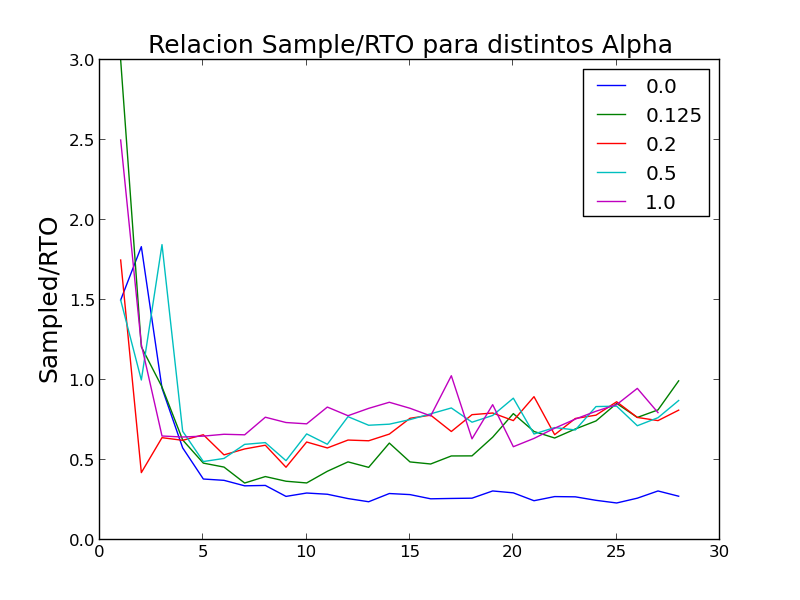
\includegraphics[width=\linewidth]{../graficos/alphad01var5drop0.png}
\caption{Relación Sample/RTO, $\beta$ = 0.25}\label{fig:alpha-var5-drop0}
\end{minipage}
\hfill
\begin{minipage}{0.5\linewidth}
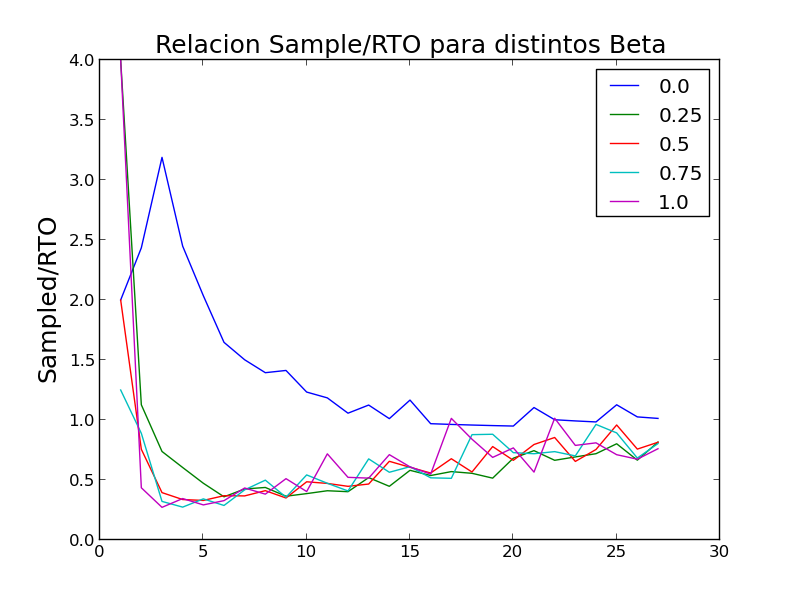
\includegraphics[width=\linewidth]{../graficos/betad01var5drop0.png}
\caption{Relación Sample/RTO, $\alpha$ = 0.125}\label{fig:beta-var5-drop0}
\end{minipage}
\end{figure}

\subsubsection{Varianza baja, delay alto}

\begin{figure}[H]
\begin{minipage}{0.5\linewidth}
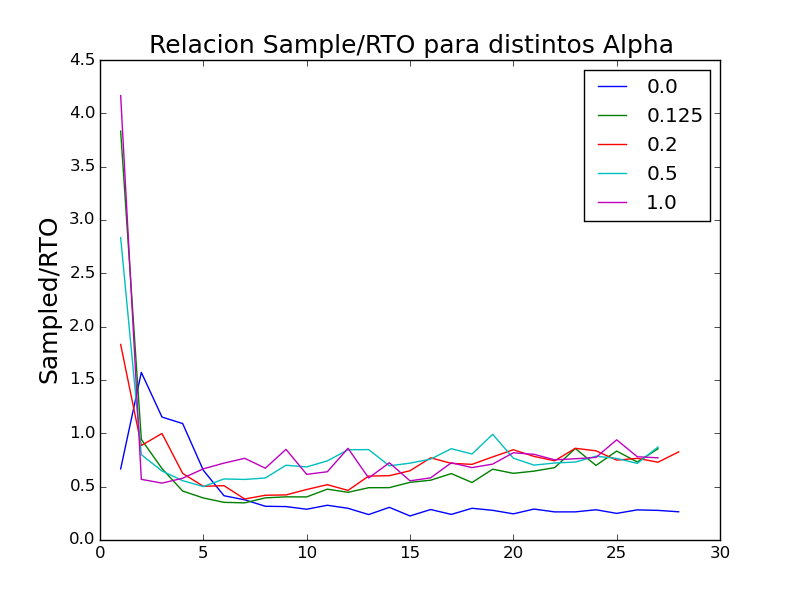
\includegraphics[width=\linewidth]{../graficos/alphad025var2drop0.png}
\caption{Relación Sample/RTO, $\beta$ = 0.25}\label{fig:alpha-var2-drop0-alto}
\end{minipage}
\hfill
\begin{minipage}{0.5\linewidth}
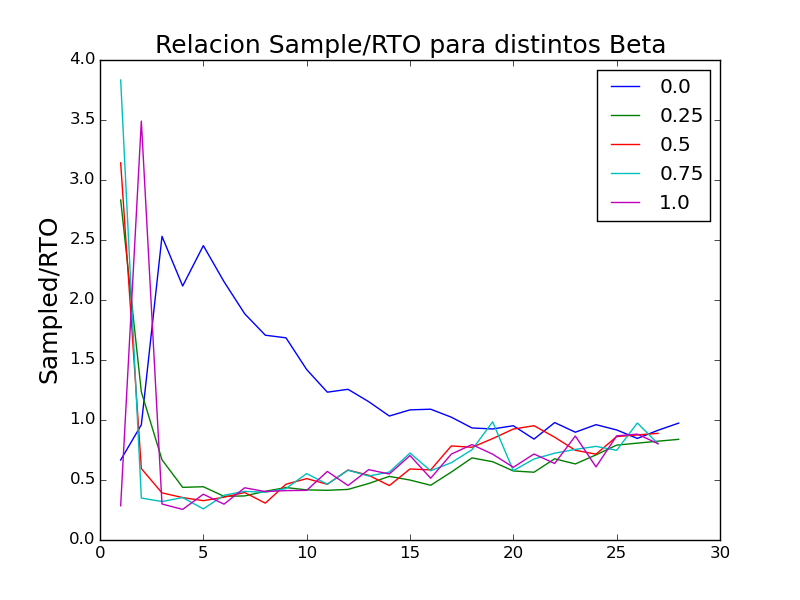
\includegraphics[width=\linewidth]{../graficos/betad025var2drop0.png}
\caption{Relación Sample/RTO, $\alpha$ = 0.125}\label{fig:beta-var2-drop0-alto}
\end{minipage}
\end{figure}

\subsubsection{Varianza alta, delay alto}

\begin{figure}[H]
\begin{minipage}{0.5\linewidth}
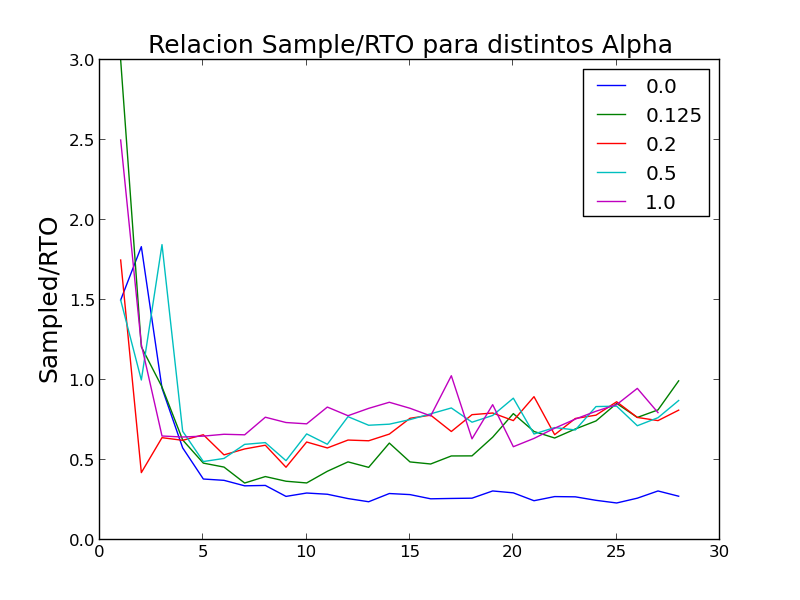
\includegraphics[width=\linewidth]{../graficos/alphad025var5drop0.png}
\caption{Relación Sample/RTO, $\beta$ = 0.25}\label{fig:alpha-var5-drop0-alto}
\end{minipage}
\hfill
\begin{minipage}{0.5\linewidth}
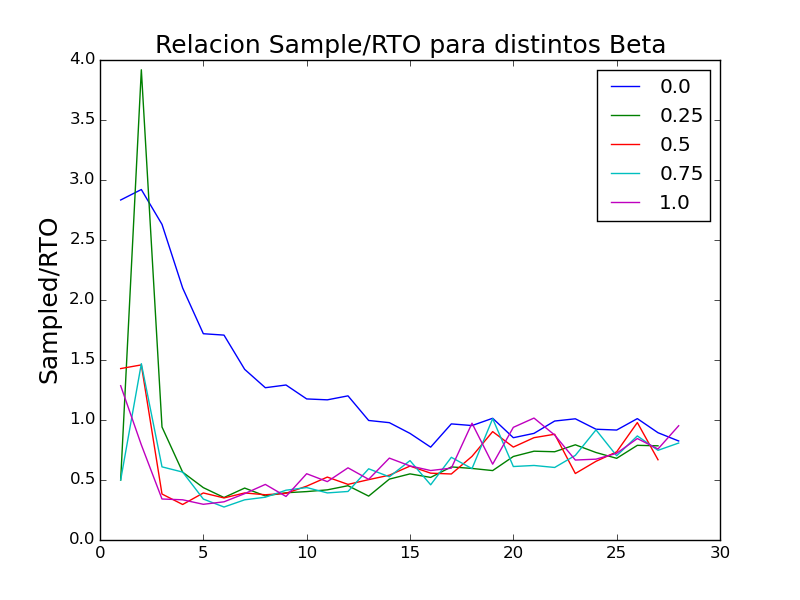
\includegraphics[width=\linewidth]{../graficos/betad025var5drop0.png}
\caption{Relación Sample/RTO, $\alpha$ = 0.125}\label{fig:beta-var5-drop0-alto}
\end{minipage}
\end{figure}

\subsection{Pérdida de paquetes baja ($p$ = 0,25)}

\subsubsection{Varianza baja, delay bajo}

\begin{figure}[H]
\begin{minipage}{0.5\linewidth}
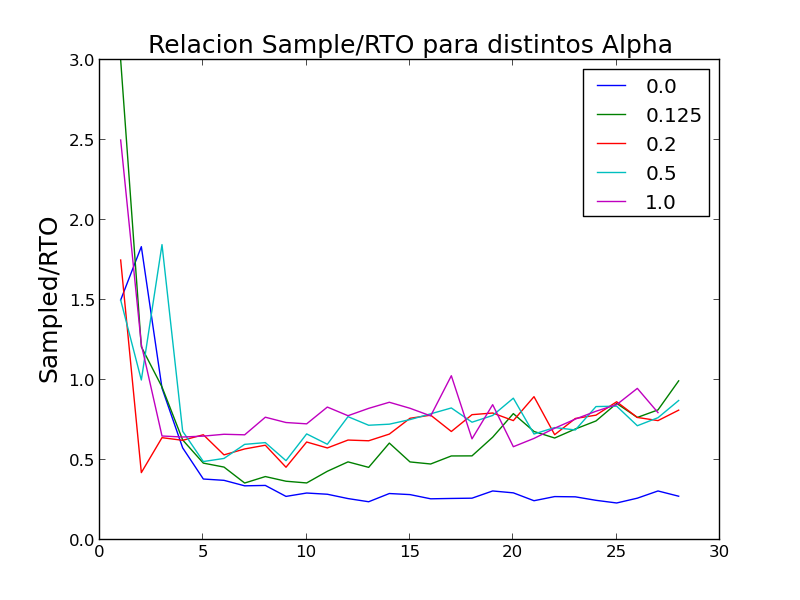
\includegraphics[width=\linewidth]{../graficos/alphad01var2drop25.png}
\caption{Relación Sample/RTO, $\beta$ = 0.25}\label{fig:alpha-var2-drop25}
\end{minipage}
\hfill
\begin{minipage}{0.5\linewidth}
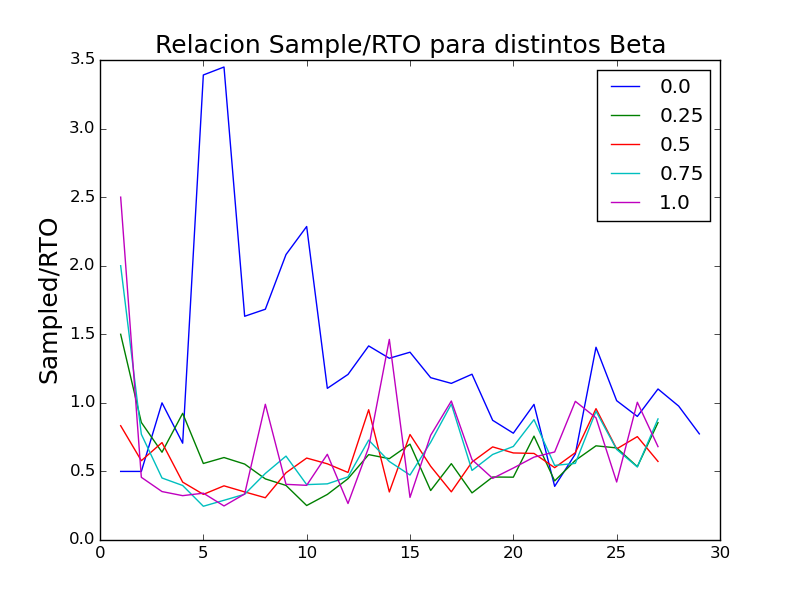
\includegraphics[width=\linewidth]{../graficos/betad01var2drop25.png}
\caption{Relación Sample/RTO, $\alpha$ = 0.125}\label{fig:beta-var2-drop25}
\end{minipage}
\end{figure}

\subsubsection{Varianza alta, delay bajo}

\begin{figure}[H]
\begin{minipage}{0.5\linewidth}
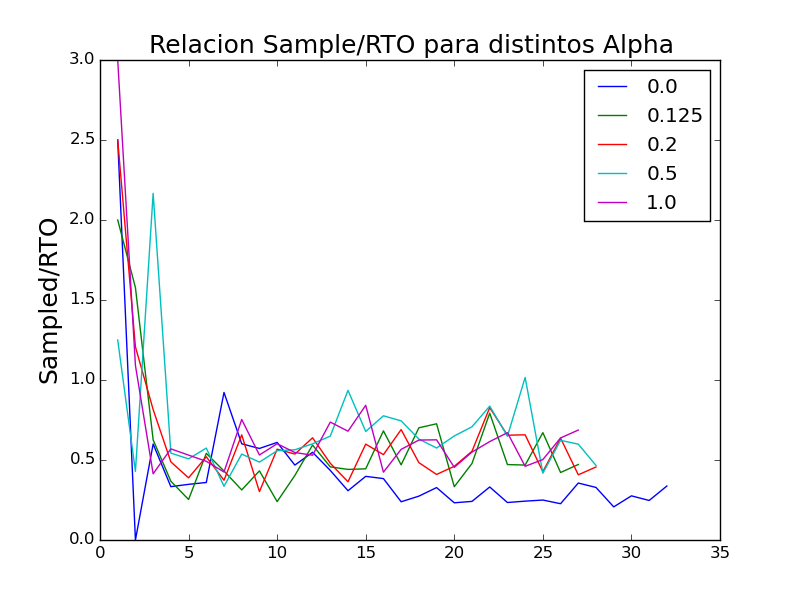
\includegraphics[width=\linewidth]{../graficos/alphad01var5drop25.png}
\caption{Relación Sample/RTO, $\beta$ = 0.25}\label{fig:alpha-var5-drop25}
\end{minipage}
\hfill
\begin{minipage}{0.5\linewidth}
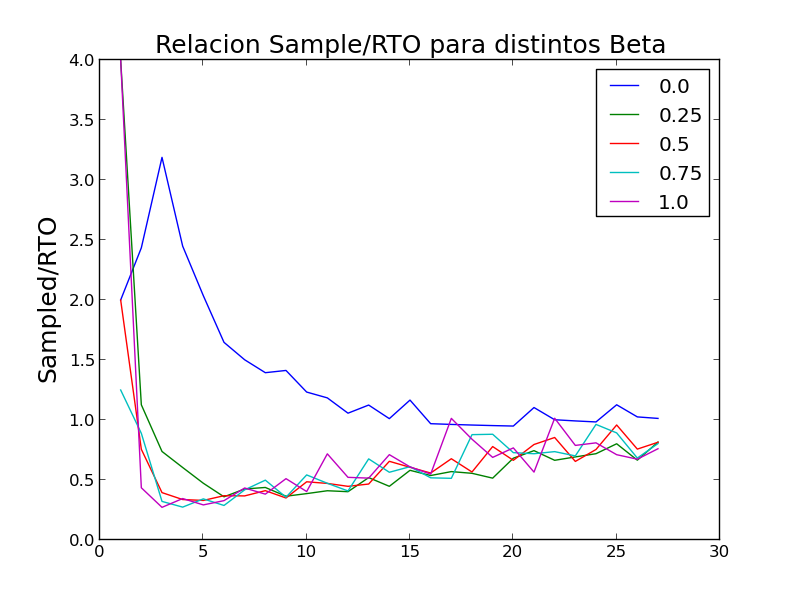
\includegraphics[width=\linewidth]{../graficos/betad01var5drop25.png}
\caption{Relación Sample/RTO, $\alpha$ = 0.125}\label{fig:beta-var5-drop25}
\end{minipage}
\end{figure}

\subsubsection{Varianza baja, delay alto}

\begin{figure}[H]
\begin{minipage}{0.5\linewidth}
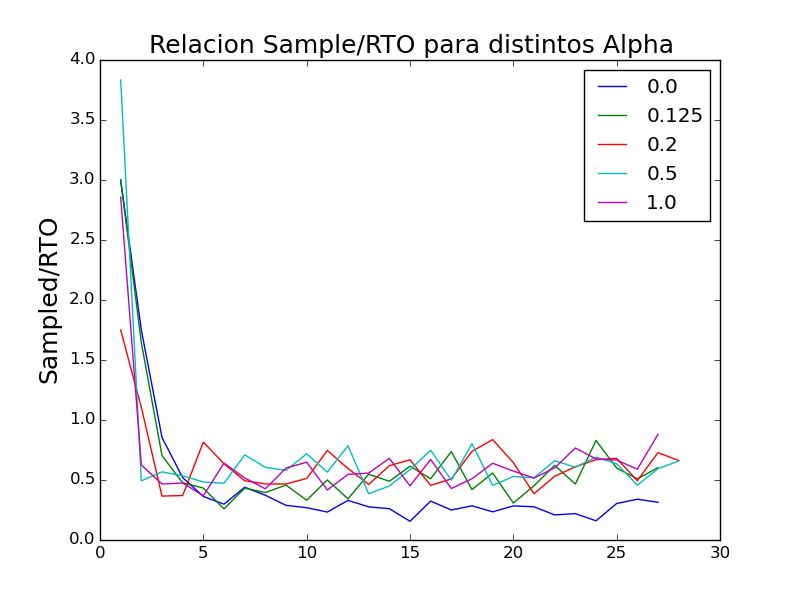
\includegraphics[width=\linewidth]{../graficos/alphad025var2drop25.png}
\caption{Relación Sample/RTO, $\beta$ = 0.25}\label{fig:alpha-var2-drop25-alto}
\end{minipage}
\hfill
\begin{minipage}{0.5\linewidth}
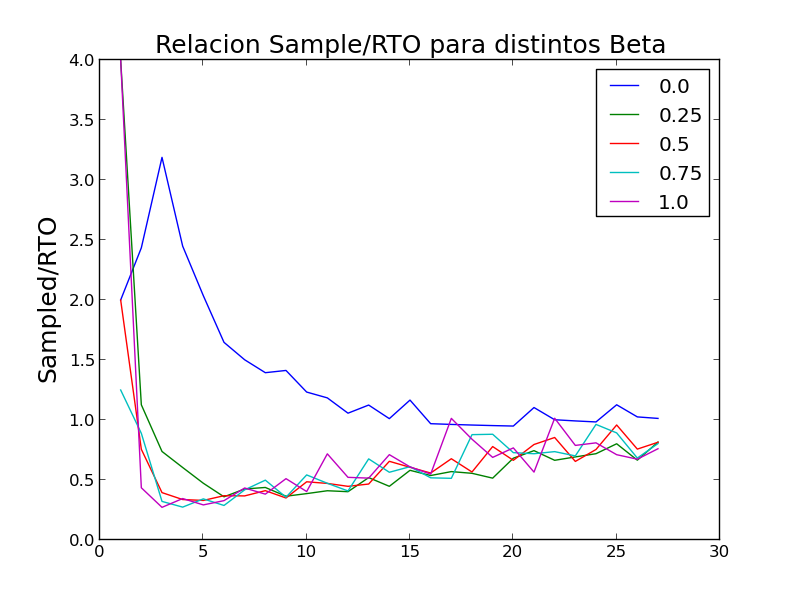
\includegraphics[width=\linewidth]{../graficos/betad025var2drop25.png}
\caption{Relación Sample/RTO, $\alpha$ = 0.125}\label{fig:beta-var2-drop25-alto}
\end{minipage}
\end{figure}

\subsubsection{Varianza alta, delay alto}

\begin{figure}[H]
\begin{minipage}{0.5\linewidth}
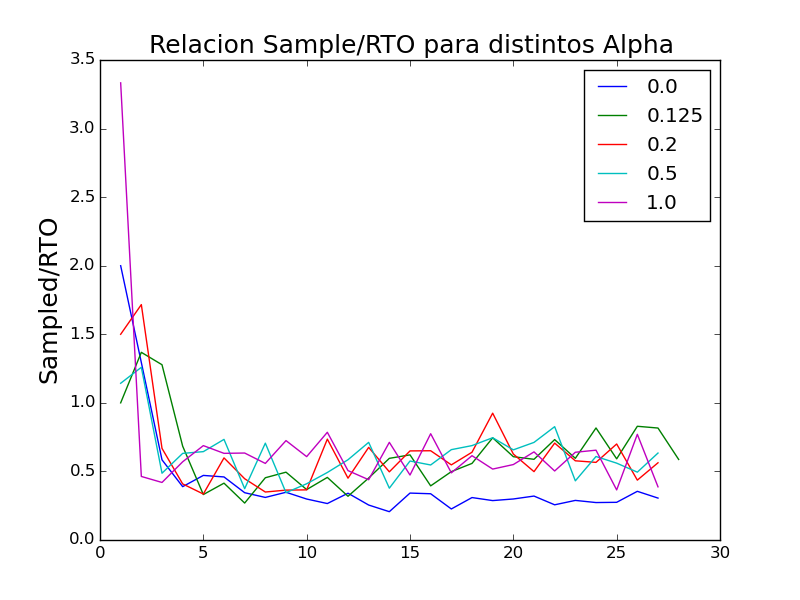
\includegraphics[width=\linewidth]{../graficos/alphad025var5drop25.png}
\caption{Relación Sample/RTO, $\beta$ = 0.25}\label{fig:alpha-var5-drop25-alto}
\end{minipage}
\hfill
\begin{minipage}{0.5\linewidth}
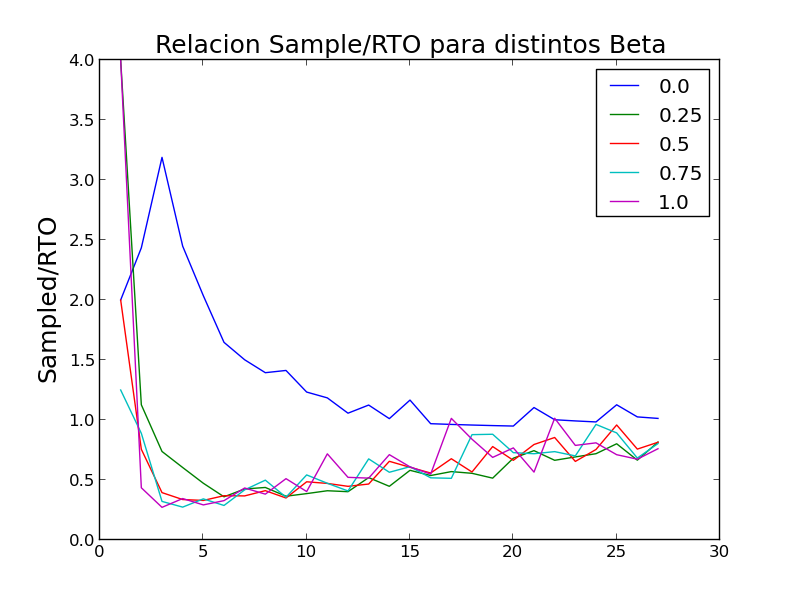
\includegraphics[width=\linewidth]{../graficos/betad025var5drop25.png}
\caption{Relación Sample/RTO, $\alpha$ = 0.125}\label{fig:beta-var5-drop25-alto}
\end{minipage}
\end{figure}

\subsection{Pérdida de paquetes alta ($p$ = 0,5)}

\subsubsection{Varianza baja, delay bajo}

\begin{figure}[H]
\begin{minipage}{0.5\linewidth}
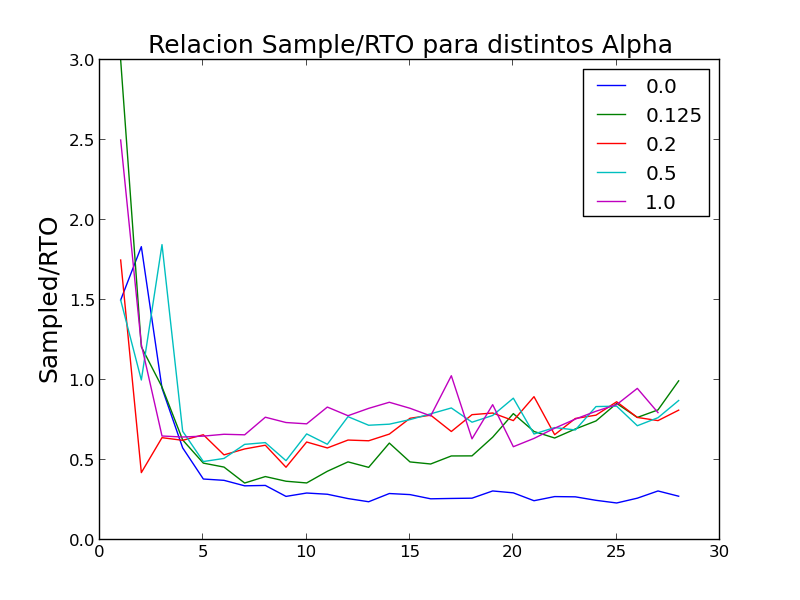
\includegraphics[width=\linewidth]{../graficos/alphad01var2drop50.png}
\caption{Relación Sample/RTO, $\beta$ = 0.25}\label{fig:alpha-var2-drop50}
\end{minipage}
\hfill
\begin{minipage}{0.5\linewidth}
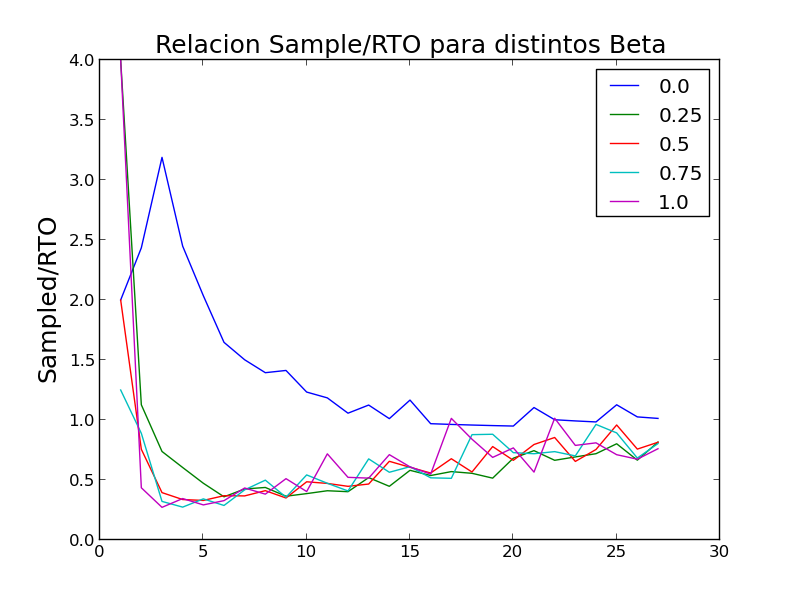
\includegraphics[width=\linewidth]{../graficos/betad01var2drop50.png}
\caption{Relación Sample/RTO, $\alpha$ = 0.125}\label{fig:beta-var2-drop50}
\end{minipage}
\end{figure}

\subsubsection{Varianza alta, delay bajo}

\begin{figure}[H]
\begin{minipage}{0.5\linewidth}
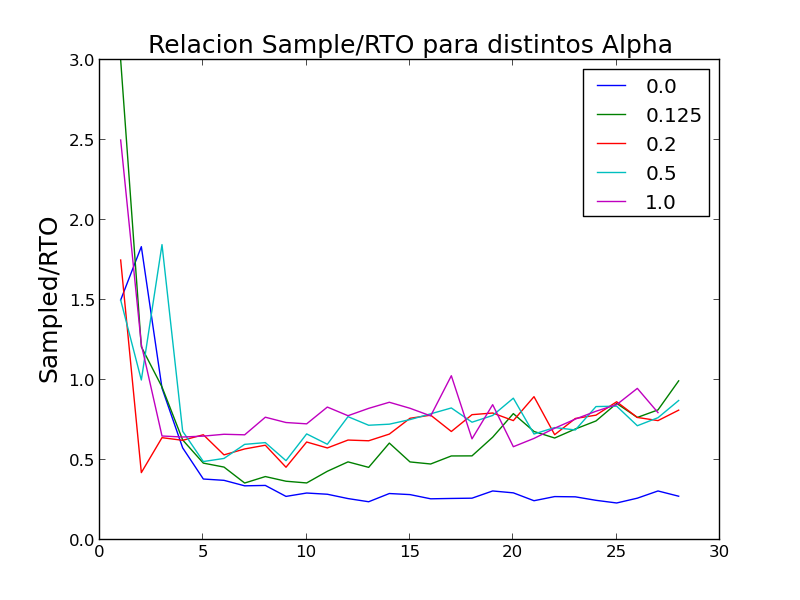
\includegraphics[width=\linewidth]{../graficos/alphad01var5drop50.png}
\caption{Relación Sample/RTO, $\beta$ = 0.25}\label{fig:alpha-var5-drop50}
\end{minipage}
\hfill
\begin{minipage}{0.5\linewidth}
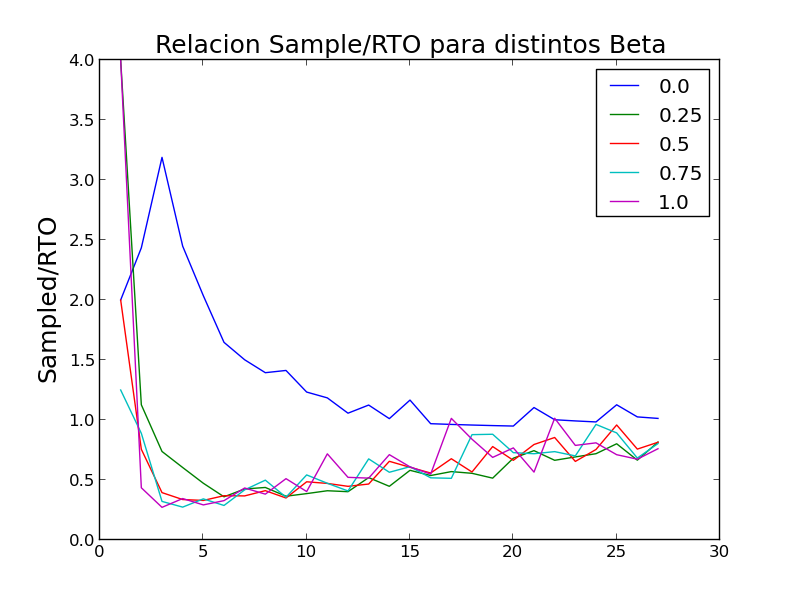
\includegraphics[width=\linewidth]{../graficos/betad01var5drop50.png}
\caption{Relación Sample/RTO, $\alpha$ = 0.125}\label{fig:beta-var5-drop50}
\end{minipage}
\end{figure}

\subsubsection{Varianza baja, delay alto}

\begin{figure}[H]
\begin{minipage}{0.5\linewidth}
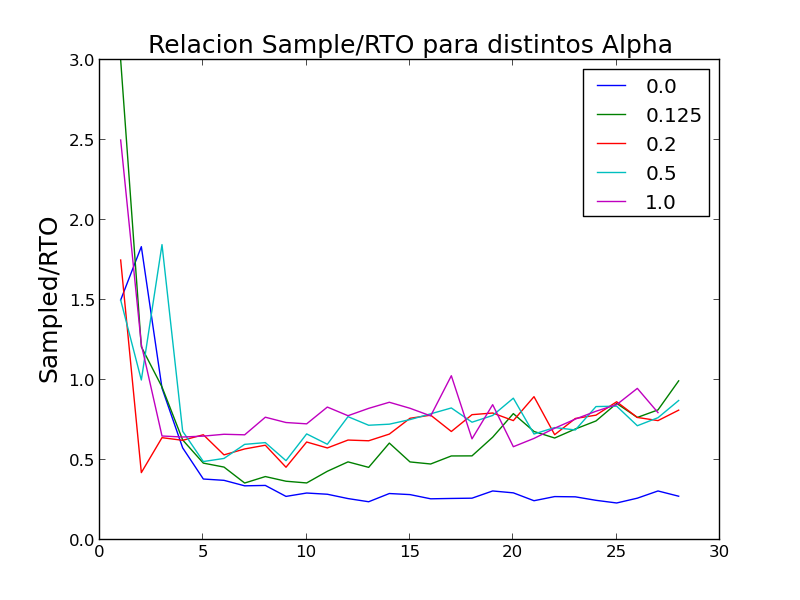
\includegraphics[width=\linewidth]{../graficos/alphad025var2drop50.png}
\caption{Relación Sample/RTO, $\beta$ = 0.25}\label{fig:alpha-var2-drop50-alto}
\end{minipage}
\hfill
\begin{minipage}{0.5\linewidth}
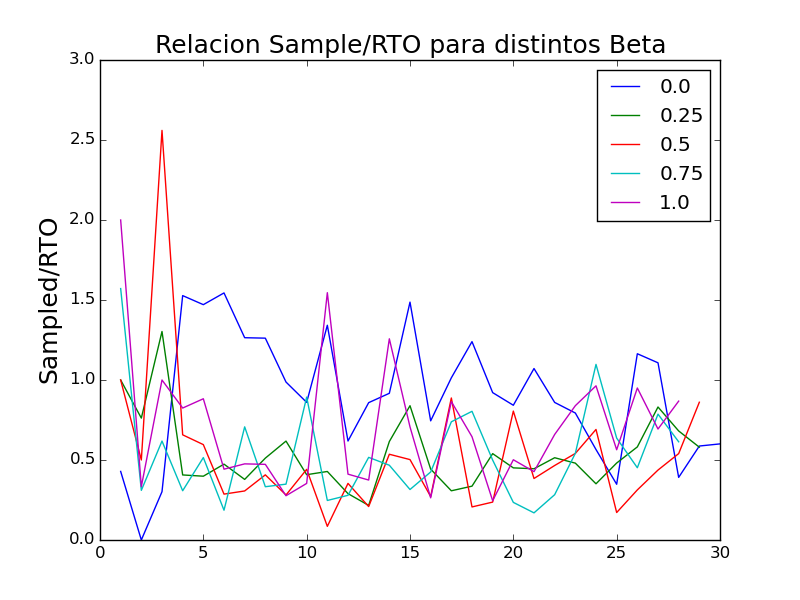
\includegraphics[width=\linewidth]{../graficos/betad025var2drop50.png}
\caption{Relación Sample/RTO, $\alpha$ = 0.125}\label{fig:beta-var2-drop50-alto}
\end{minipage}
\end{figure}

\subsubsection{Varianza alta, delay alto}

\begin{figure}[H]
\begin{minipage}{0.5\linewidth}
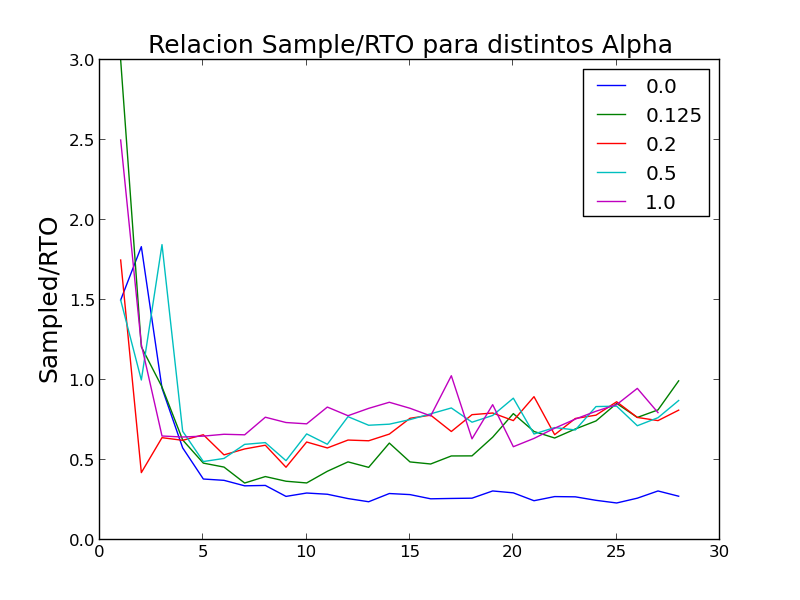
\includegraphics[width=\linewidth]{../graficos/alphad025var5drop50.png}
\caption{Relación Sample/RTO, $\beta$ = 0.25}\label{fig:alpha-var5-drop50-alto}
\end{minipage}
\hfill
\begin{minipage}{0.5\linewidth}
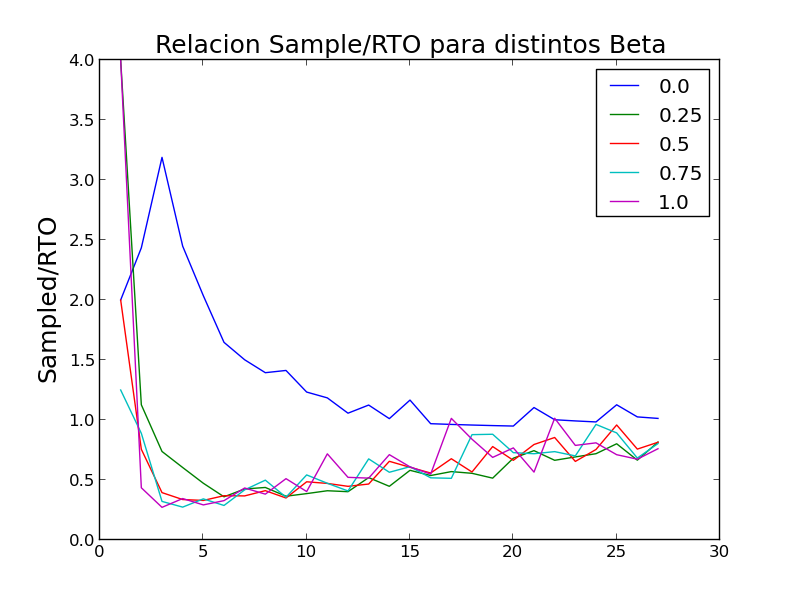
\includegraphics[width=\linewidth]{../graficos/betad025var5drop50.png}
\caption{Relación Sample/RTO, $\alpha$ = 0.125}\label{fig:beta-var5-drop50-alto}
\end{minipage}
\end{figure}